\section{Data Taking}
\label{sec:data taking}

The results reported here are based on data taken in October 2012 
during a dedicated LHC proton fill (3216)
with the very special beam properties described in the previous section.

The vertical RPs approached the beam centre to only 3 times the beam width, $\sigma_{y}$, resulting in an acceptance for $|t|$-values down to $6 \times 10^{-4}\,\rm GeV^{2}$. The exceptionally close distance was possible due to the low beam intensity in this special beam operation: each beam contained only two colliding bunches and one non-colliding bunch for background monitoring, each with $10^{11}$ protons. A novel collimation strategy was applied to keep the beam halo background under control. As a first step, the primary 
collimators (TCP) in the LHC betatron cleaning insertion (point 7) scraped the beam down to $2\,\sigma_{y}$; then the collimators were retracted to $2.5\,\sigma_{y}$, thus creating a $0.5\,\sigma_{y}$ gap between
the beam edge and the collimator jaws. With the halo strongly suppressed 
and no collimator producing showers by touching the beam, the RPs at 
$3\,\sigma_{y}$ were operated in a background-depleted environment for about one 
hour until the beam-to-collimator gap was refilled by diffusion, as 
diagnosed by the increasing RP trigger rate (Figure~\ref{fig:overview}). When the background conditions
had deteriorated to an unacceptable level, the beam cleaning procedure was repeated, again followed by a quiet data-taking period.
This entire sequence was iterated 6 times until the luminosity had decreased 
from initially $1.8\times10^{27}\,\rm cm^{-2}s^{-1}$ to 
$0.4\times10^{27}\,\rm cm^{-2}s^{-1}$
at which point the data yield was considered as too low. 
During the 9 hour long fill, an integrated luminosity of $20\,\rm \mu b^{-1}$ 
was accumulated in 6 data sets corresponding to the calm periods 
between the cleaning operations. 

Due to an anti-collision protection system, the top and the bottom pots of a 
vertical RP unit could not approach each other close enough to be both at a 
distance of $3\,\sigma_{y} = 780\,\mu$m from the beam centre. Therefore a 
configuration with one RP diagonal (45 top -- 56 bottom) at $3\,\sigma_{y}$ (``close diagonal'') and the other (45 bottom -- 56 top) at 
$10\,\sigma_{y}$ (``distant diagonal'') was chosen. The distant diagonal provides a systematic comparison at larger $|t|$-values.
The horizontal RPs were only needed for the data-based alignment and therefore placed at a safe distance of $10\,\sigma_{x} \approx 7.5$\,mm, close enough to have an overlap with the vertical RPs (Figure~\ref{fig:rpsketch}, right).

The events collected were triggered by a logical \textit{OR} of: inelastic 
trigger (activity in either arm of T1 or T2), double-arm proton trigger 
(coincidence of any RP left of IP5 and any RP right of IP5) and zero-bias trigger (random bunch crossings) for calibration purposes.

In the close and distant diagonals a total of 190k and 162k elastic event candidates have been tagged, respectively.


\begin{figure*}
\begin{center}
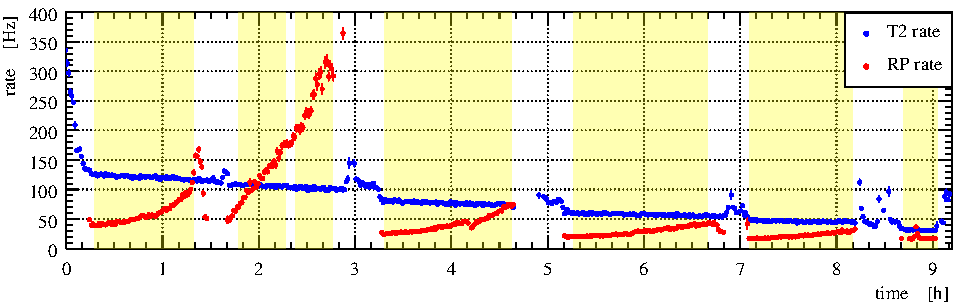
\includegraphics{fig/trigger_rate.pdf}
\vskip-3mm
\caption{%
Trigger rates as a function of time from the beginning of the run. The T2 rate (blue) is roughly proportional to luminosity, while the RP rate (red) is in addition sensitive to beam-halo level. The yellow bands represent periods of uninterrupted data taking.
}
\label{fig:overview}
\end{center}
\end{figure*}
